\chapter{Constructing Disjunctive Normal Form Expressions}\label{ch:dnf}

% definition and characteristics of DNF -> why is it so interesting
A disjunctive normal form (DNF) formula is defined to be a disjunction of at least one conjunction of at least one literal~\citep{aizenstein}.
Each literal is either a negated or a non negated variable. 
Moreover each variable can be interpreted as \(g: X -> \lbrace0,1\rbrace\), for any Boolean expression \(X\)~\citep{davey}.

% every function can be a DNF -> motivation
Every classification concept that is representable as a Boolean function, is convertible into an equivalent DNF,
using logical equivalences like for example the De Morgan's laws \(a \vee b = \overline{a \wedge b}\)~\citep{davey}.
Moreover DNFs are canonical normal forms of Boolean functions, meaning that every Boolean function has exactly one representation as a full DNF,
that is definite except for variations based on associativity and commutativity of the logical conjunctions~\citep{davey}.
Though, there is no guarantee for a DNF representation to be compact.
~\cite{aizenstein} prove that the correct DNF representation of a subject cannot only be found in exponential time,
but for large groups of issues even in only polynomial time.

% minimized DNFs
A DNF can be minimized using tools like Karnaugh maps or the Quine–McCluskey algorithm~\citep{allender}.
A classic minimization could for example be the summarizing of `\((a \wedge b)\vee(a \wedge \overline{b})\)' to `\(a\)'.
Even though the algorithm for finding the minimal DNF is NP-complete and will therefore not be implemented here,
the optional solution can be approximated by the greedily collecting the prime implicants and
always adding the conjunction to the disjunction next, that covers the most remaining positive samples~\citep{allender}.

% motivation
DNFs are widely spread in machine learning and still subject to further research,
as they provide easy to interpret decision functions as representations for many real-world concepts, even in complex scientific contexts~\citep{aizenstein}.
Whereas a conjunctive normal form formula is comparatively hard to interpret for humans, since it appears less often in nature.
Thus, I decided to extend the the conjunctive classification rules of the set covering machine into DNF expressions.
A `full DNF' furthermore would have every variable appear in every conjunction, however those special DNFs do in general not result from the SCM.\

% using DNFs in the SCM
So far the SCM only constructs pure conjunctions or pure disjunctions.
Yet, in classification tasks with disjunctly scattered samples, pure conjunctions are
unable to give accurate classifications and DNFs are strongly needed.
After commenting on the general concept and its Julia implementation in \autoref{sec:conc},
different approaches to optimize the \(SCM_{DNF}\) are presented:
first by adjustments on the input parameters (\autoref{sec:adjustingParam}) and later by
making use of equally optimal base classifiers (\autoref{sec:ties}).

%%%%%%%%%%%%%%%%%%%%%%%%%%%%%%%%%%%%%%%%%%%%%%%%%%%%%%%%%%%%%%%%%%%%%%%%%%%%%%%%%%%%%%%%%%%%
\section{Concept and Implementation}\label{sec:conc}

While, in the algorithm of~\cite{haussler88}, every sample is per definition correctly covered by the first conjunction,
canceling the need of having multiple conjunctions, with~\cite{marchand02} introducing the hyperparameter \(p\), this situation changed.
Now it is not uncommon anymore for a conjunction not to cover all positive samples.
By the use of an ensemble of conjunctions and the linking of those by one big disjunction,
more positive samples can be covered by the classification rule and feasible results can be achieved, even for data sets, as in \autoref{fig:twoReg}, with
extremely disjunct decision regions within a class.

\begin{figure}[ht]
    \centering
    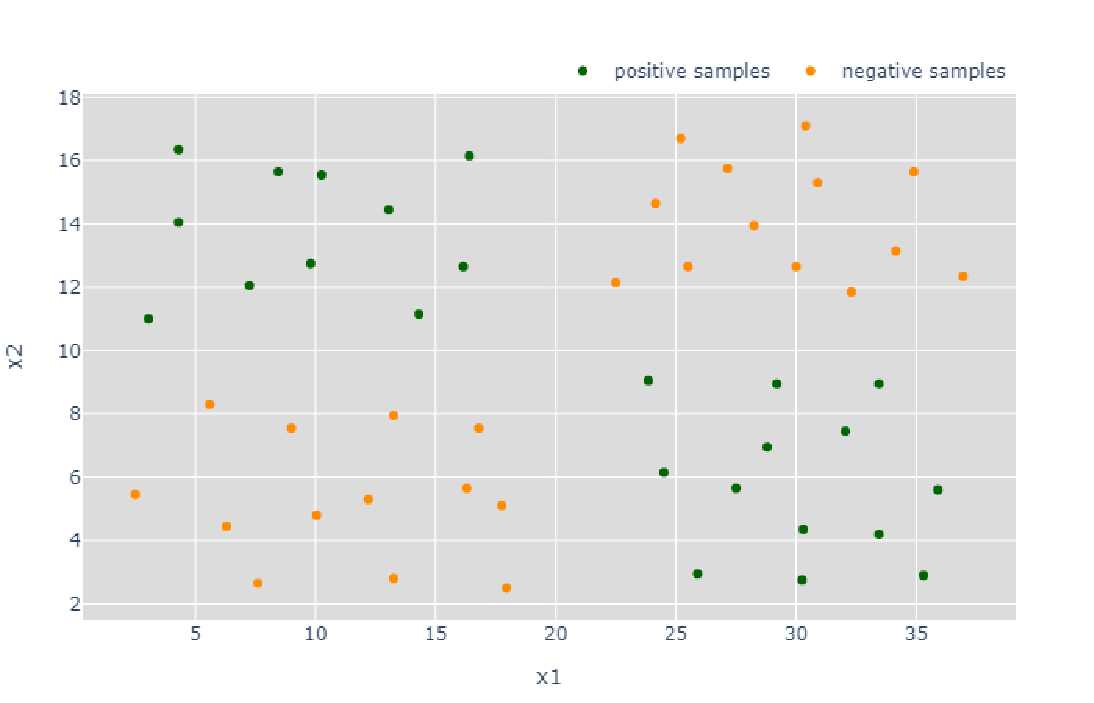
\includegraphics[width=0.85\columnwidth]{figures/two_reg.pdf}
    \caption{Data set with positive samples that scatter distinctly into two decision regions.}\label{fig:twoReg}
\end{figure}

The schematic algorithm to build DNF classification rules is depicted in \autoref{code:SCM_DNF}, its Julia implementation can be found in \autoref{julia:buildDnf}.
Here \(sC\) defines the maximum number of base classifiers within each conjunction and \(sD\) the maximum number of conjunctions within the disjunction.
\(minConjSize\) on the other hand sets a minimum usefulness requirement for conjunctions in order for them to be included into the DNF.\
The code of the conjunctive SCM can directly be integrated into this algorithm and in general does not need to be changed at all,
as the algorithm solely extends the conjunctive SCMs rule to a whole set of rules and thus creates an \(SCM_{DNF}\).
By the mechanisms of greedily picking optimal conjunctions for the disjunction, the generated DNF will even be in a somewhat, yet not
guaranteed to be optimal, minimal form~\citep{allender}.

\begin{algorithm}[ht]
    \KwIn{\(S\), \(p\), \(sC\), \(sD\), \(minConjSize\)}
    conjunctions = \(\emptyset\) \\
    \While{\(\exists\) misclassified positive sample AND length of conjunctions \(< sD\)}{
        conj = whole, and maximal big, conjunctive classifier generated by \autoref{julia:buildConj} with the parameters \(S\), \(p\) and \(sC\) \\
        Predict the labels of each sample using conj. \\
        \If{conj = \(\emptyset\) OR \{positive samples covered by conj\} < \(minConjSize\)}{
            Break loop.
        }
        \(S = S -\) positive samples covered by conj \\
        conjunctions = conjunctions \(\cup\) conj \\
    }
    Return conjunctions.
    \caption{Basic algorithm to build a DNF classifier from conjunctive classifiers.}\label{code:SCM_DNF}
\end{algorithm}

The \texttt{build\_dnf} algorithm is actually really similar to the algorithm of building a conjunctive SCM, with the main differences being
that conjunctions are collected, instead of single base classifiers, and in every iteration the samples that are classified as positive,
instead of negative, get deleted from the data set, as this classification is now final.
This is caused by the uneven behavior of conjunctions and disjunctions, that comes especially clear when observing
the ways each rule type classifies samples in \autoref{julia:classify}.
By placing conjunctions nested in a disjunction, the asymmetric behavior is somehow balanced.

%%%%%%%%%%%%%%%%%%%%%%%%%%%%%%%%%%%%%%%%%%%%%%%%%%%%%%%%%%%%%%%%%%%%%%%%%%%%%%%%%%%%%%%%%%%%
\section{Adjusting the Algorithms Parameters}\label{sec:adjustingParam}

To ensure that the algorithm is able to produce good results for various data sets,
the parameters \(p\), \(sD\), \(sD\) and \(minConjSize\), that can be adjusted independently, are implemented.

%%%%%%%%%%%%%%%%%%%%%%%%%%%%%%%%%%%%%%%%%%%%%%%%%%%%%%%%%%%%%%%%%%%%%%%%%%%%%%%%%%%%%%%%%%%%
\subsection{Early Stopping Points}

A DNF will usually perform better than a pure conjunction when it comes to classifying the training data, as it has more possibilities to cover the data points.
However that is not necessarily the case, when it comes to classifying unknown test data.
The possibility to link multiple conjunctions into a DNF gives the SCM the ability to extremely
over-fit the classifier to the training data --- way more than a normal conjunctive SCM ever could.
As overfitting of the training data leads to a high generalization error on test data and therefore
an overall bad performance of the classifier, it is crucial to find a good balance between high accuracies on
training data and high generalizability.

The input parameters \(sC\in \mathbb{N}\), \(sD\in \mathbb{N}\) and \(minConjSize\in \mathbb{N}\) are used to help with this exact problem.
They are early stopping points, meaning that they force the classification rule building process to stop,
even if there could still be a base classifier or conjunction added.
\(sC\) in particular limits the DNF to a k-NDF with \(k = sC\).
While \(sC\) and \(sD\) leads to a process termination simply by providing a hard upper limit to the maximum number of
base classifiers or conjunctions, \(minConjSize\) has the softer approach.
It stops the algorithm whenever an `optimal' conjunction is picked, covering so few positive samples, 
that it does not actually help with identifying a new decision region.

As the main goal is to find and characterize all decision regions of the data set, I focus on the use of the \(minConjSize\) parameter.
If the SCM is for example executed on a data set that actually has five disjunct decision regions, with ten positive samples each, along with some random scattering,
The algorithm should not terminate after it found \(n\) of those decision regions because \(sD\) forced it to stop.
Instead it is supposed to find all five regions and then stop, because the sixth region it found
is too small and loose to classify at least \(minConjSize\) additional positive samples as positiv.
As a consequence, both, \(sC\) and \(sD\), are in general set to the comparatively high standard value of 10 and
focus on the adjustment of \(minConjSize\).

\begin{figure}
    \centering
    \begin{subfigure}{\textwidth}
        \centering
        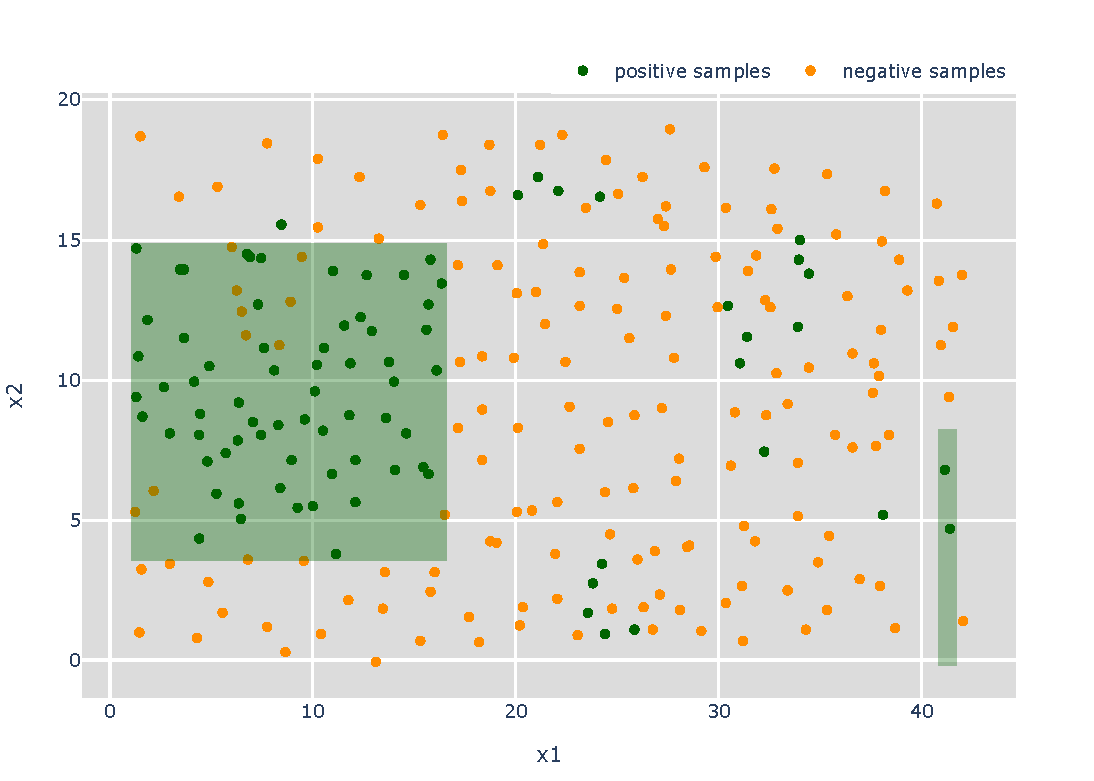
\includegraphics[width=0.85\columnwidth]{figures/complex_pattern_conj_size_1.pdf}
        \caption{\(minConjSize = 1\).}
    \end{subfigure}
    \hfill
    \begin{subfigure}{\textwidth}
        \centering
        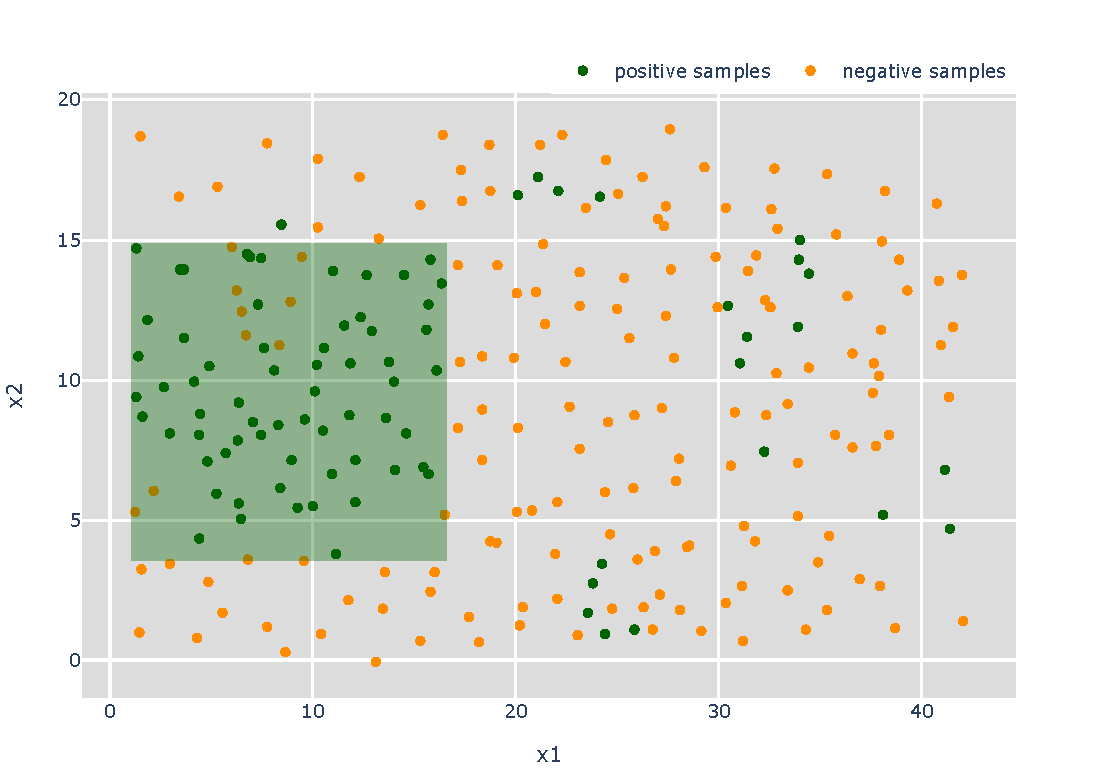
\includegraphics[width=0.85\columnwidth]{figures/complex_pattern_conj_size_5.pdf}
        \caption{\(minConjSize = 5\).}
    \end{subfigure}
    \caption{Classification rule for an artificial data set with one main data regions and some additional small ones.
    The algorithms use different minimum conjunction sizes. Both use \(p = 2\).}\label{fig:complexPatternConjSize}
\end{figure}

A simple visualization of the benefits of restricting the use of small conjunctions 
to achieve a better generalizable model is displayed in \autoref{fig:complexPatternConjSize}, where
the SCM with \(minConjSize = 1\) identifies an additional decision region, in an area that does in fact not contain one. 
An elaborate study on the adjustment of the \(minConjSize\) parameter for gene expression data can be found in \autoref{subsec:studySCM}.
There, the data set's vast amount of features and comparatively small quantity of samples facilitate overfitting extremely well and thus make the use of an early stopping point
especially interesting.
In general a good \(minConjSize\) should be relative to the number of samples, leading to a higher value for big data sets and a lower
value for data sets with only a few total samples available.

%%%%%%%%%%%%%%%%%%%%%%%%%%%%%%%%%%%%%%%%%%%%%%%%%%%%%%%%%%%%%%%%%%%%%%%%%%%%%%%%%%%%%%%%%%%%
\subsection{Penalty Value p}

Additionally the penalty value \(p\in \mathbb{R}\) can, and should, be adjusted according to the algorithm's use case and the characteristics of the data set.
While a low \(p\) value, especially \(p < 1\), avoids the misclassification of negative samples as positive ones and therefore increases the algorithm's specificity,
a high value of \(p\) avoids the misclassification of positive samples as negative ones, thus increasing the algorithm's sensitivity.
This results in comparatively small decision regions when working with a low \(p\) and bigger ones when working with a higher \(p\).

~\cite{haussler88} suggests too keep the amount of misclassified negative samples as small as possible when using a DNF,
as misclassified positive samples can still be covered by following conjunctions, however once a negative sample is misclassified by
a conjunction, this error cannot be corrected anymore.
But unfortunately when using data dependent rays as features, low \(p\) values usually do not work out too well,
because, in contrast to data dependent interval, the selection of a rays is done without knowing what other rays can be selected next.
Therefore \(p\) has to be adjusted carefully and cannot be placed arbitrarily high or low.

\begin{figure}
    \centering
    \begin{subfigure}{\textwidth}
        \centering
        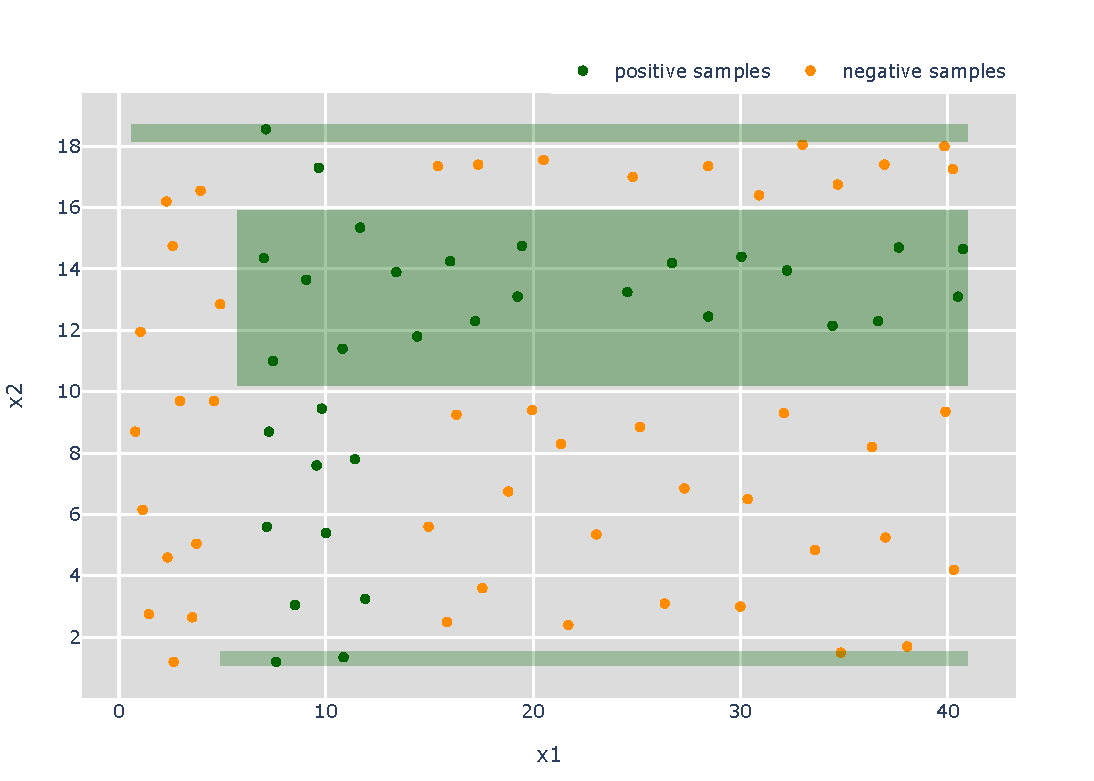
\includegraphics[width=0.85\columnwidth]{figures/cross_1.pdf}
        \caption{\(p = 1\).}
    \end{subfigure}
    \hfill
    \begin{subfigure}{\textwidth}
        \centering
        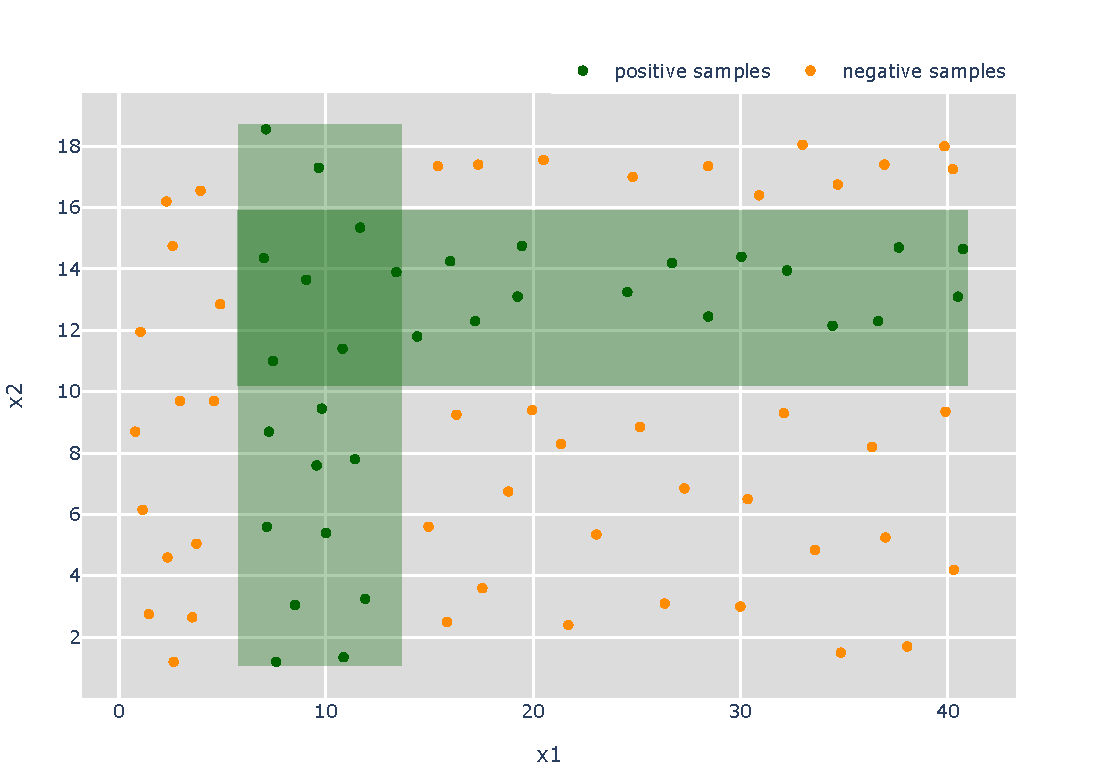
\includegraphics[width=0.85\columnwidth]{figures/cross_1_5.pdf}
        \caption{\(p = 1.5\).}
    \end{subfigure}
    \caption{Classification rule for an artificial data set with two orthogonal decision regions. Both models use a \(minConjSize\) of \(1\).}\label{fig:crossP}
\end{figure}

This can be illustrated using the example of \autoref{fig:crossP}:
Here the algorithm with \(p=1.5\) finds the reasonable decision rule `\texttt{IF (x2 > 10.35 AND x2 < 15.77 AND x1 > 5.95) OR (x1 < 13.42 AND x1 > 6.0) THEN class 1}',
however the algorithm with \(p=1\) finds a far less suitable one.
While they both have the same first conjunction, the more risky algorithm then chooses the ray `x1 < 13.42', which
the other algorithm did not choose.
This is because, without knowing that there is a perfect ray `x1 > 6.0' that can be chosen next,
this ray evaluates to 12 new positive samples to be correctly classified and 14 negative samples to be misclassified.
So even though the situation seems quite obvious for a human observer, rays often decide for
more defensive selections of rays next to the data set's borders, like the SCM with \(p=1\) did here.

When using \(p = \inf\) the SCM always selects the conjunction first, that is guaranteed to cover all positive samples, without considering
the misclassified negative samples at all.
This leads to a \(SCM_{DNF}\) that would always only consist of one single conjunction and
is therefore an unnecessary option to consider in this thesis.

As it is quite complicated to come up with a mathematical formula to compute the penalty parameter \(p\)
that maximizes the classifiers accuracy, I instead focus on balancing the
specificity and the sensitivity of a DNF classifier.
This configuration does in general not maximize the accuracy, yet it ensures that the weaker class has a reasonable accuracy, too. % self driving car and pedestrian

The usefulness of a base classifier, and therefore the possibility that it is chosen, is defined as
\[Q - p \cdot R = \text{`correctly classified negative samples'} - p \cdot \text{`misclassified positive samples'}\]
The parameter \(p\) therefore defines the weight balance between positive and negative samples.
By setting \(p\) as \(\frac{|\text{`neg.\ samples'}|}{|\text{`pos.\ samples'}|}\) this balance is approximately evened out,
as \[\text{`correctly classified neg.\ samples'} - \frac{|\text{`neg.\ samples'}|}{|\text{`pos.\ samples'}|} \cdot \text{`misclassified pos.\ samples'} \approx 0\]
In this way an SCM with approximately the same sensitivity and specificity can be created.
However the formula requires \(sC\) and \(sD\) being high enough and \(minConjSize\) being small enough, so the ratio will not be influenced by these factors.
Moreover the training and the test data's class 1 to class 0 samples ratios need to be round about the same.
This is for example provided when the test data is generated by a cross-validation (see \autoref{sec:evalMethods}).
The formula will later be tested on the `german' data set in \autoref{subsec:german}, as this data set has an especially uneven ratio of classes,
as well as on the gene expression data sets in \autoref{subsec:studySCM}.

%%%%%%%%%%%%%%%%%%%%%%%%%%%%%%%%%%%%%%%%%%%%%%%%%%%%%%%%%%%%%%%%%%%%%%%%%%%%%%%%%%%%%%%%%%%%
\section{Making Use of Ties}\label{sec:ties}

% idea
Often times, when comparing different thresholds, operators or features, the SCM will come across base classifiers that have the exact same score.
Those base classifiers can be considered as `ties'.
~\cite{kestler06} already suggested that `break[ing] ties of equivalent greedy solutions'~\citep[p. 296]{kestler06} may increase the SCM's robustness.
I now want to investigate on this idea in the context of DNF decision rules.

Usually only one of those options is picked and the other one is discarded, however the \(SCM_{DNF}\)
seems like a good framework for actually making use of those ties, as the SCM can
store both base classifiers, complete the conjunction with the first base classifier and then append the second base classifier and its conjunction using a logical-OR.\
Additionally it has to be considered, that there might also be three or more ties at once and new ties might appear
while the SCM is still resolving another tie.

In order to work with ties, some adaptions to the Julia code are needed:
In \texttt{inspect\_\\single\_feature\ (NominalFeature)} and \texttt{find\_border} not only one optimal threshold, but all thresholds,
that share the highest score, need to be returned, as depicted in \autoref{julia:tiesCollect1}.
Similarly, in \texttt{inspect\_single\_feature\ (NumericalFeature)}, if the optimal ray using \(\geq\)
and the optimal ray using \(\leq\) have equal scores, both will be returned (see \autoref{julia:tiesCollect2}).
As \texttt{find\_base\_classifier} compares the base classifiers of the different features and returns the optimum, ties can also occur here
and need to be collected by a procedure like the one in \autoref{julia:tiesCollect3}.
However the main difference is in the \texttt{build\_conjunction} function.
Here all ties from the subfunctions get collected.
One base classifier is then used immediately while the others are returned to \texttt{build\_dnf} together with their
histories, i.e.\ all base classifiers that were selected in this conjunction so far.
There they will then be stored and used as an input parameter for the next \texttt{build\_conjunction} calls.
This is illustrated in \autoref{julia:buildDnfTies}.
In particular \texttt{popfirst!} ensures that always latest found tie is used for the next conjunction.
Whenever \texttt{build\_conjunction} is now called with some preselected base classifiers from a recent tie,
these base classifiers are used as the classifier's preamble and the algorithm continues to extend their conjunction.
However these ties still need to pass the \(minConjSize\) test or otherwise the algorithm is immediately terminated.
This modified \texttt{build\_conjunction} function can be found in \autoref{julia:buildConjTies}, while the old one is depicted in \autoref{julia:buildConj}.

But in fact, the base classifiers are only helpful in very few cases.
For example in the situation of \autoref{fig:tiesA}, when using \(p=1\), there will be the tie between the rays \(x < \alpha\) and \(x < \beta\).
These ties are definitely worth tracking.
The same goes for \autoref{fig:tiesB}, where all four rays \(x < \alpha\), \(x > \alpha\), \(y < \alpha\) and \(y > \alpha\)
have the same usefulness score and can therefore be considered as ties.
Yet, here the selection might already be unlucky: if one for example selects \(x < \alpha\) first, followed by \(y < \alpha\)
to complete the conjunction, the selection of the previous tie \(y < \alpha\) as the first ray for the next conjunction would lead to 
an immediate end of the algorithm with only `\texttt{IF \(x < \alpha\) AND \(y < \alpha\) THEN class 1}' as the classification rule,
without the consideration of the positive samples within \texttt{`\(x > \alpha\) AND \(y > \alpha\)}'.
In the case of the data set depicted in \autoref{fig:tiesC}, using ties is rather counterproductive,
as only one ray is needed, \(x < \alpha\) or \(y > \alpha\).
Therefore it is quite useless to memorize the second ray as well.
Moreover in the situation of \autoref{fig:tiesD}, all four marked rays have the same scores when using a penalty value of 1.
Yet, again luck for the correct order of choosing rays is needed.
If for example \(x < \alpha\) is chosen first, followed by \(x < \beta\), \(x < \gamma\) and finally \(x < \delta\),
the SCM ends up with a pretty bulky classification rule that barely has any significance.

In general it is often the case that there are many ties present, however most of them are comparatively useless and will only make the algorithm terminate.
This is due to the fact that samples that are classified by the current conjunction are removed from the data set before continuing
to resolve the tie situations.
In the scenarios \autoref{fig:tiesB}, \autoref{fig:tiesC}, \autoref{fig:tiesD} and many more this means that the investigation on the tie does usually not at all equal the investigation on the currently optimal ray.
A study about the performance of an SCM that utilizes ties when working on gene expression data can be found in \autoref{subsec:studySCM}.

\begin{figure}
    \centering
    \begin{subfigure}[b]{0.5\textwidth}
        \centering
        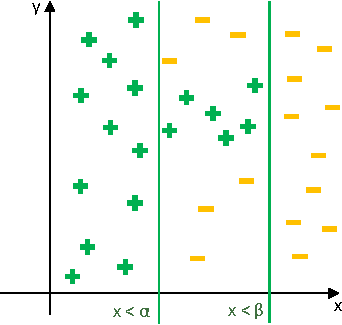
\includegraphics[width=\textwidth]{figures/ties_A.pdf}
        \caption{Situation A.}\label{fig:tiesA}
    \end{subfigure}%
    \begin{subfigure}[b]{0.5\textwidth}
        \centering
        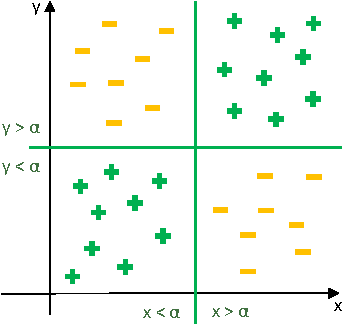
\includegraphics[width=\textwidth]{figures/ties_B.pdf}
        \caption{Situation B.}\label{fig:tiesB}
    \end{subfigure}
    \begin{subfigure}[b]{0.5\textwidth}
        \centering
        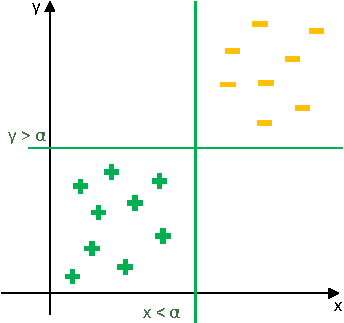
\includegraphics[width=\textwidth]{figures/ties_C.pdf}
        \caption{Situation C.}\label{fig:tiesC}
    \end{subfigure}%
    \begin{subfigure}[b]{0.5\textwidth}
        \centering
        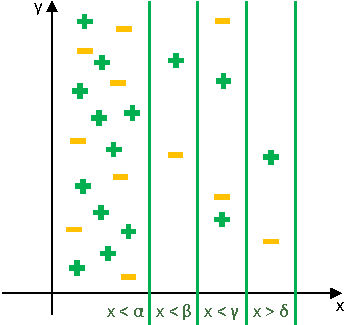
\includegraphics[width=\textwidth]{figures/ties_D.pdf}
        \caption{Situation D.}\label{fig:tiesD}
    \end{subfigure}
    \caption{Scenarios, in which the utilization of ties is more or less useful.}\label{fig:ties}
\end{figure}

I additionally tried an implementation, in which a tie base classifier, that does not fulfill the algorithms requirements
of correctly classifying at least one positive and one negative sample, does not lead to an immediate termination of the algorithm,
but instead the tie is discarded and the algorithm goes on with the next iteration.
However this algorithm led to extremely high execution times, as even on data sets with only a few hundred samples and features
thousands of ties were checked and discarded again, making the algorithm so slow that it is simply not feasible to use on bigger data sets.